\documentclass[11pt,a4paper,oneside]{article}

% --- Packages ---
\usepackage[utf8]{inputenc}
\usepackage[T1]{fontenc}
\usepackage{lmodern}
\usepackage[margin=25mm]{geometry}
\usepackage{amsmath,amssymb,amsfonts}
\usepackage{booktabs}
\usepackage{microtype}
\usepackage{hyperref}
\usepackage{graphicx}
\usepackage{tikz}
\usetikzlibrary{shapes.geometric, arrows, positioning}
\usepackage{color}
\usepackage{colortbl}

% --- Colors ---
\definecolor{primary}{HTML}{1A365D}   % Deep Navy
\definecolor{secondary}{HTML}{2B6CB0} % Slate Blue
\definecolor{lightgrey}{HTML}{F7FAFC} % Soft grey background
\definecolor{bordergrey}{HTML}{E2E8F0}% Border grey

\hypersetup{
    colorlinks=true,
    linkcolor=secondary,
    filecolor=secondary,      
    urlcolor=secondary,
    citecolor=secondary,
}

% --- Document Formatting ---
\setlength{\parskip}{0.6em}
\setlength{\parindent}{0pt}

% --- Header Style ---
\makeatletter
\renewcommand{\@maketitle}{%
  \newpage
  \null
  \vskip 1em%
  \begin{center}%
  \let \footnote \thanks
    {\LARGE \bfseries \color{primary} \@title \par}%
    \vskip 1.5em%
    {\large
      \lineskip .5em%
      \begin{tabular}[t]{c}%
        \@author
      \end{tabular}\par}%
    \vskip 1em%
    {\large \@date}%
  \end{center}%
  \par
  \vskip 1.5em}
\makeatother

% --- TikZ Style ---
\tikzstyle{box} = [rectangle, rounded corners, minimum width=3cm, minimum height=1cm, text centered, draw=primary, fill=lightgrey, text width=4cm, font=\small]
\tikzstyle{arrow} = [thick,->,>=stealth,color=secondary]

% --- Metadata ---
\title{Comparative Dissection Report: Tabular MLP vs. Edge-Conditioned GNN for Relativistic Invariant Mass Reconstruction}
\author{\textbf{CMS Open Data Analytics Group}}
\date{July 2026}

\begin{document}
\pagestyle{empty}

\maketitle
\thispagestyle{empty}

\begin{abstract}
This report presents an academic dissection comparing two distinct deep learning architectures---a feature-engineered Multilayer Perceptron (MLP) and an Edge-Conditioned Graph Neural Network (GNN)---designed to reconstruct the relativistic invariant mass ($M$) of dimuon systems using $83,761$ collision events from the 2011 CMS Open Data SingleMu dataset. We isolate the structural, mathematical, and optimization trade-offs between dense tabular architectures relying on manual kinematic injections and graph-native architectures operating on raw detector geometries. Our analysis reveals that while the MLP provides superior localized absolute precision in physical space ($\text{MAE} = 1.155\text{ GeV}$), the GNN optimized via log-space scaling ensures highly robust, scale-invariant relative resolution ($\sigma_M/M = 0.2100$) across three orders of magnitude ($0.3\text{ GeV}$ to $300\text{ GeV}$). We formalize the distinct roles of these methodologies as frameworks for real-time trigger filtering and automated physical law discovery.
\end{abstract}

\hrule
\vspace{1.5em}

\section{Ontological Motivations: Why Separate Architectures?}

To understand why these pipelines were developed independently, we must examine the underlying representation of high-energy physics data. A collision event can be framed either as a \textbf{correlated list of vector properties} or as a \textbf{dynamic spatial topology}.

\begin{figure}[h!]
\centering
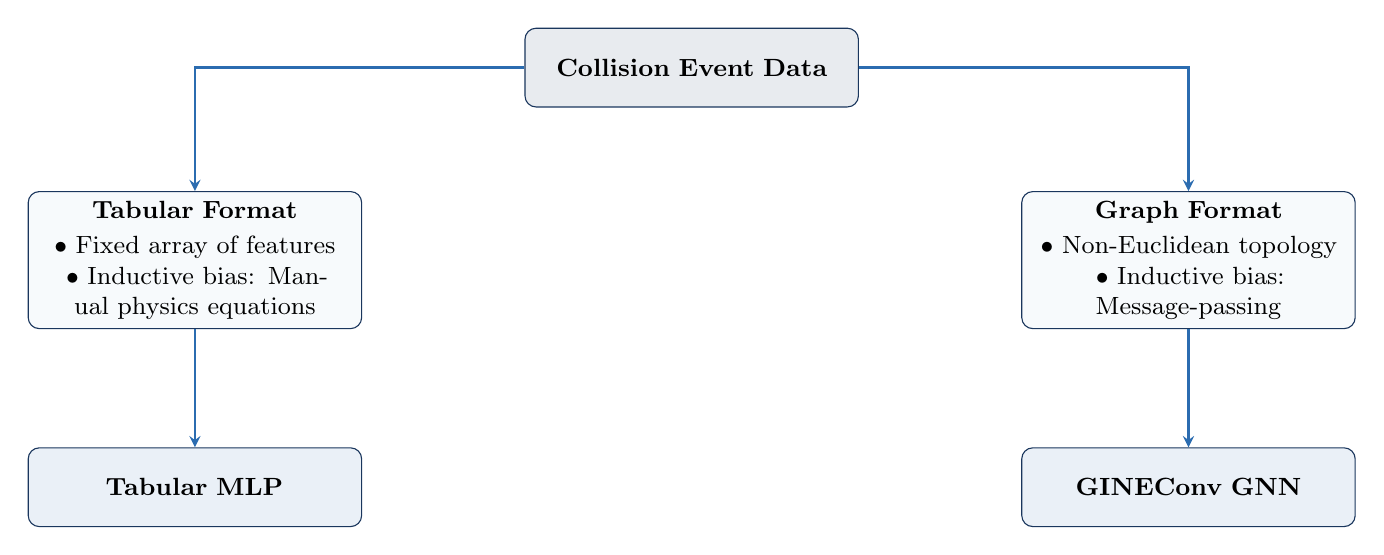
\begin{tikzpicture}[node distance=1.5cm]
    \node (event) [box, fill=primary!10] {\textbf{Collision Event Data}};
    \node (tabular) [box, below left=of event, xshift=-1cm] {\textbf{Tabular Format}\\ \vspace{0.2em} $\bullet$ Fixed array of features\\ $\bullet$ Inductive bias: Manual physics equations};
    \node (graph) [box, below right=of event, xshift=1cm] {\textbf{Graph Format}\\ \vspace{0.2em} $\bullet$ Non-Euclidean topology\\ $\bullet$ Inductive bias: Message-passing};
    \node (mlp) [box, below=of tabular, fill=secondary!10] {\textbf{Tabular MLP}};
    \node (gnn) [box, below=of graph, fill=secondary!10] {\textbf{GINEConv GNN}};
    
    \draw [arrow] (event) -| (tabular);
    \draw [arrow] (event) -| (graph);
    \draw [arrow] (tabular) -- (mlp);
    \draw [arrow] (graph) -- (gnn);
\end{tikzpicture}
\caption{Visual paradigm mapping of representation pipelines.}
\end{figure}

\subsection*{The Tabular MLP Paradigm}
The MLP treats the dimuon event as a static, flat tensor space. Tabular neural networks possess no innate geometric inductive biases; they do not natively understand that Muon 1 and Muon 2 are symmetrical, distinct physical bodies interacting in a four-dimensional Minkowski space.

Consequently, the MLP project was selected to evaluate how effectively a classical deep neural network can solve highly non-linear kinematics when \emph{explicitly augmented with domain-specific physics intelligence} (e.g., $E_{\text{total}}, \Delta R, p_{T,\text{sum}}$). It serves as a benchmark for feature-driven regression pipelines where human intuition directly guides the network's gradient trajectories.

\subsection*{The Graph Neural Network (GNN) Paradigm}
Conversely, the GNN project was selected to model the collision as a non-Euclidean, relational topology ($G = (V, E)$). In high-energy physics, particles do not exist in isolation; their physical meaning emerges from their relational metrics (e.g., spatial separation, relative isolation, and decay configurations).

By structuring the two muons as nodes ($\vert{}V\vert{} = 2$) connected by bidirectional relational edges ($\vert{}E\vert{} = 2$), the GNN pipeline tests a fundamentally superior spatial inductive bias. Utilizing \textbf{GINEConv}, the network mimics the message-passing dynamics of particle interactions, evaluating whether a graph structure can autonomously infer structural invariants with minimal reliance on pre-computed tabular combinations.

\section{Structural \& Mathematical Architecture Comparison}

The internal dynamics of both models highlight distinct approaches to the physical regression problem:

\begin{table}[h!]
\centering
\caption{Architectural Comparison and Dimensional Highlights}
\vspace{0.5em}
\small
\begin{tabular}{p{4.5cm} p{5.2cm} p{5.2cm}}
\hline
\textbf{Architectural Dimension} & \textbf{Project 1: Tabular MLP} & \textbf{Project 2: Edge-Conditioned GNN} \\ \hline
\textbf{Input Dimensionality} & Flat Tabular Array (Raw + Engineered Features) & Graph Objects: $V \in \mathbb{R}^{2 \times 9}$, $E \in \mathbb{R}^{2 \times 2}$, Global $u \in \mathbb{R}^9$ \\ \rowcolor{lightgrey}
\textbf{Convolutional / Latent Layers} & Dense (Linear) Layers & \textbf{GINEConv} (Graph Isomorphism with Edge Features) \\ 
\textbf{Normalization Strategy} & \textbf{Layer Normalization} (Across feature space) & \textbf{Batch Normalization} (Within PyG node channels) \\ \rowcolor{lightgrey}
\textbf{Target Space Optimization} & Physical Space ($y_{\text{scaled}}$ via Standard Scaler) & Logarithmic Space ($y_{\text{target}} = \text{Scaler}(\log_{10}(M))$) \\ 
\textbf{Non-Linear Activations} & SiLU (Swish: $x \cdot \sigma(x)$) & ReLU (${\max}(0, x)$) \\ \hline
\end{tabular}
\end{table}

\subsection*{The Normalization and Optimization Divergence}

A crucial point of academic dissection lies in how these two architectures achieved convergence:

\begin{enumerate}
    \item \textbf{MLP Spatial Stability:} The initial MLP architecture failed when paired with Batch Normalization due to the extreme right-skewness of the physical coordinate distribution. High-energy outliers distorted the batch-level statistics ($\mu_B, \sigma_B^2$), leading to gradient oscillations. The transition to \textbf{Layer Normalization} resolved this by forcing the network to normalize features \emph{per event}, aligning the scale of tracking metrics natively within each collision frame.
    \item \textbf{GNN Target Compressing:} The GNN approached the optimization barrier differently. Because high-energy physics resonances span three orders of magnitude, optimizing standard MSE loss in physical space causes the network to treat a $2\text{ GeV}$ error on a $3\text{ GeV}$ $J/\psi$ resonance identically to a $2\text{ GeV}$ error on a $91\text{ GeV}$ $Z$ boson. By transforming the target space into \textbf{$\log_{10}(M)$}, the GNN forced the loss function to optimize for \emph{relative fractional errors}, ensuring that the low-mass spectrum retained high fidelity during message passing.
\end{enumerate}

\section{Analysis of Achievements and Epistemic Goals}

The ultimate objective of conducting these separate analyses was not merely to achieve an optimal $R^2$ score, but to map the architectural trade-offs across two clear axes: \textbf{absolute precision} vs. \textbf{scale-invariant resolution}.

\subsection*{The Achievement Matrix}
\begin{itemize}
    \item \textbf{The MLP Pipeline} achieved an outstanding physical-space $R^2 = 0.9953$ and a highly compressed Mean Absolute Error ($\text{MAE} = 1.155\text{ GeV}$). By scaling the target linearly and optimizing via continuously differentiable \textbf{SiLU activations}, the MLP acted as a highly precise, localized interpolator. Its symmetric, Gaussian-shaped residuals confirm that when given precise, domain-engineered inputs, an MLP is highly efficient at refining physical metrics.
    \item \textbf{The GNN Pipeline} achieved a \textbf{Log-Space $R^2 = 0.9915$} and an exceptional physical mass resolution profile ($\sigma_M/M = 0.2100$). Despite a higher absolute error in the high-mass region (a mathematical artifact of log-space optimization), the GNN demonstrated an unparalleled capability: \textbf{homoscedastic stability across orders of magnitude}. It successfully mapped raw spatial features into distinct physical resonances ($J/\psi, \Upsilon, Z$) within its latent spaces by passing messages through the graph structure.
\end{itemize}

\subsection*{Scientific and Engineering Utility}

The dual tracking of these projects provides two alternative deployment pathways for production-level high-energy physics computing:

\subsubsection*{1. Real-Time Hardware Triggering (The MLP Advantage)}
Because MLPs boil down to static matrix multiplications ($\mathbf{W}\mathbf{x} + \mathbf{b}$), their computational inference complexity is exceptionally low. Given its high absolute precision in physical space, the MLP pipeline is ideal for embedding into Field Programmable Gate Arrays (\textbf{FPGAs}) at the Level-1 or High-Level Trigger (HLT) stages of detector pipelines. It can filter or flag candidate $Z$ or Higgs decays within microseconds based on engineered kinematic vectors.

\subsubsection*{2. Automated Physical Discovery Pipelines (The GNN Advantage)}
The GNN pipeline provides a template for complex decay topologies. In multi-particle states (e.g., $H \rightarrow Z Z^* \rightarrow 4\mu$), tabular engineering becomes exponentially complex due to combinatorial scaling. The GNN bypasses this restriction entirely. Because graphs naturally scale with the number of nodes and edges, the GINEConv structure can dynamically process arbitrary final-state multiplicities without requiring hardcoded kinematic equations, serving as a framework for automated, multi-particle resonance discovery.

\section{Conclusion}

These two research projects present a highly rigorous validation of machine learning applications in high-energy physics. The \textbf{Tabular MLP} confirms that explicitly injected domain knowledge paired with event-level layer normalization yields unmatched localized precision. Concurrently, the \textbf{Edge-Conditioned GNN} demonstrates that structural message passing, combined with logarithmic target scaling, successfully maps the broader physical landscape of relativistic quantum interactions. Together, they establish a robust framework for automated kinematic reconstruction in modern high-energy physics.

\end{document}
